% !TeX spellcheck = en_GB
\documentclass[11pt]{article}

\usepackage[type1]{libertine}
\usepackage[a4paper]{geometry}
\usepackage{amsmath, amsthm, amssymb} 
\usepackage{parskip}
\usepackage{tabularx}
\usepackage[english]{babel}
\usepackage{enumitem}
\usepackage{gensymb}
\usepackage{bm}
\usepackage{graphicx}
\usepackage{xcolor}
\usepackage{float}
\usepackage{wrapfig}
\usepackage{cancel}
\usepackage{multicol}
\usepackage{commath} % Provides good differentials

\usepackage[titletoc,title,toc,page]{appendix}
\usepackage{hyperref}
\hypersetup{
	pdftitle={The Double Atwood Machine},
	pdfauthor={Sun Yudong},
	bookmarksnumbered=true,
	bookmarksopen=true,
	bookmarksopenlevel=2,
	pdfstartview=Fit,
	pdfpagemode=UseOutlines,
	colorlinks=true,
	linkcolor=black,
	filecolor=magenta,      
	urlcolor=blue
}

\newenvironment{multicolFigure}
{\par\medskip\noindent\minipage{\linewidth}}
{\endminipage\par\medskip}
% https://tex.stackexchange.com/questions/12262/multicol-and-figures

\newenvironment{amatrix}[1]{%
	\left(\begin{array}{@{}*{#1}{c} | c@{}}
	}{%
	\end{array}\right)
}						% https://tex.stackexchange.com/a/2238
\usepackage{blkarray}	% https://tex.stackexchange.com/a/59519
\usepackage{mathtools}	% https://tex.stackexchange.com/a/103993

\title{The Double Atwood Machine}
\author{Sun Yudong\\Hwa Chong Institution}

\begin{document}
	\maketitle
	\section*{Problem Statement}
	\begin{wrapfigure}{r}{3.5cm}
		\centering
		\vspace{-0.7cm}
		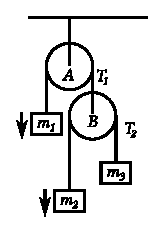
\includegraphics[width=3cm]{problem.eps}
		\label{fig:atwood}
	\end{wrapfigure}
	In the figure, masses $m_2$ and $m_3$ are connected by a light string over a light, frictionless pulley $B$. The axle of pulley $B$ is connected by a light string over a light, frictionless pulley $A$ to a mass $m_1$. Pulley $A$ is suspended from the ceiling by an attachment to its axle. The system is released from rest. We want to find the acceleration of each of the masses, and the tensions $T_1$ and $T_2$.
	
	Consequently, what do our expressions give for the special case of $m_2 = m_3$ and $m_1 = m_2 + m_3$? Is this reasonable?
	
	(You can also find this problem in Morin's \textit{Introductory Classical Mechanics})
	
	\section*{The Newton Way}
	Our first step in tackling this is to write \textit{Newton's 2\textsuperscript{nd} Law} for all the masses: \\ (Taking down as positive)
	\begin{align}
		m_1 a_1 &= m_1 g - T_1  \label{eqn:m1a1} \\
		m_2 a_2 &= m_2 g - T_2  \label{eqn:m2a2} \\
		m_3 a_3 &= m_3 g - T_2  \label{eqn:m3a3} 
	\end{align}
	Since pulley $B$ is massless, there is no net force on the pulley. Or thinking about it in the opposite manner, if there is any net force on the pulley, the pulley would have infinite acceleration, which does not make any physical sense. 
	
	We thus deduce:
	\begin{equation}
		T_1 = 2 T_2 \label{eqn:tension}
	\end{equation}
	
	Counting the variables, we realize there are 5 unknowns. We are missing one equation. This is the step we apply the \textbf{the conservation of string}.
	
	\subsection*{Conservation of String}
	\begin{wrapfigure}{r}{3.5cm}
		\centering
		\vspace{-0.7cm}
		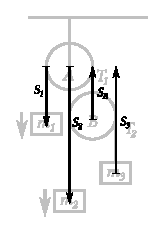
\includegraphics[width=2.9cm]{cos.eps}
		\vspace{-0.3cm}
		\caption{Double Atwood Machine}
		\label{fig:conservationOfString}
		\vspace{-3cm}
	\end{wrapfigure}

	For elaboration of the Conservation of String, refer to Appendix \ref{appdx:COS}. 	

	Assuming you have already understood the conservation of string, applying first to the right half of the set up in Figure \ref{fig:conservationOfString}:
	\begin{align}
		(S_2 - S_p) + (S_3 - S_p) &= L \notag \\
		S_2 + S_3 - 2S_p &= L \notag \\
		\dod[2]{}{t}\left(S_2 + S_3 - 2S_p\right) &= \dod[2]{}{t}L \notag\\
		a_2 + a_3 - 2a_p &= 0 \notag \\
		a_2 + a_3 &= 2a_p \label{eqn:COS1}
	\end{align}
	Now we apply the conservation of string to the left side of the set up to obtain:
	\begin{equation}
		a_1 = -a_p \label{eqn:COS2}
	\end{equation}
	Combining \eqref{eqn:COS1} and \eqref{eqn:COS2}, we get:
	\begin{equation}
		a_2 + a_3 = -2a_1 \label{eqn:COS}
	\end{equation}
	This is the last equation we need to solve the whole problem:
	\begin{align*}
		m_1 a_1 &= m_1 g - T_1  &m_1 a_1 + T_1 &= m_1 g \tag{\ref{eqn:m1a1}} \\
		m_2 a_2 &= m_2 g - T_2  &m_2 a_2 + T_2 &= m_2 g \tag{\ref{eqn:m2a2}} \\
		m_3 a_3 &= m_3 g - T_2  &m_3 a_3 + T_2 &= m_3 g \tag{\ref{eqn:m3a3}} \\
		T_1 &= 2 T_2 			&T_1 - 2 T_2 &= 0 \tag{\ref{eqn:tension}} \\
		a_2 + a_3 &= -2a_1 		&2a_1 + a_2 + a_3 &= 0 \tag{\ref{eqn:COS}}
	\end{align*}
	Since these are all linear equations (i.e. power $= 1$), we can solve these using techniques in Linear Algebra. But that is beyond the scope of this. You can refer to Appendix \ref{appdx:GES} for more information.
	
	To begin solving, we first substitute all the $T_2$ using \eqref{eqn:tension}: 
	\begin{align}
	m_1 a_1 &= m_1 g - T_1  \notag \tag{\ref{eqn:m1a1}} \\
	m_2 a_2 &= m_2 g - \frac{1}{2} T_1  \label{eqn:m2a2-2} \\
	m_3 a_3 &= m_3 g - \frac{1}{2} T_1  \label{eqn:m3a3-2} \\
	a_2 + a_3 &= -2a_1 	\notag \tag{\ref{eqn:COS}}
	\end{align}
	
	\pagebreak
	Then we write $a_1$ and $a_2$ in terms of $a_3$:
	\begin{align}
		\eqref{eqn:m2a2-2} - \eqref{eqn:m3a3-2}:~~ m_2a_2 - m_3a_3 &= m_2 g - m_3g \notag\\
		m_2a_2 &= m_2 g + m_3(a_3-g) \notag\\
		a_2 &= g + \frac{m_3}{m_2}\left(a_3 - g\right) \label{eqn:a2a3}\\
		\eqref{eqn:m1a1} - 2 \times \eqref{eqn:m3a3-2}:~~ m_1a_1 - 2m_3a_3 &= m_1 g - 2m_3g\notag\\
		m_1a_1 &= m_1 g + 2m_3(a_3-g) \notag\\
		a_1 &= g + \frac{2m_3}{m_2}\left(a_3 - g\right) \label{eqn:a1a3}
	\end{align}
	Substituting \eqref{eqn:a2a3} and \eqref{eqn:a1a3} into \eqref{eqn:COS}:
	\begin{align}
		\left[g+\frac{m_3}{m_2}\left(a_3-g\right)\right] + a_3 &= -2\left[g + \frac{2m_3}{m_2}\left(a_3 - g\right)\right] \notag\\
		g + \left(\frac{m_3}{m_2}\right)a_3 - \frac{m_3}{m_2}g + a_3 &= -2g-\left(4 \frac{m_3}{m_1}\right)a_3 + 4 \frac{m_3}{m_1}g \notag\\
		a_3\left(\frac{m_3}{m_2} + 1 + 4 \frac{m_3}{m_1}\right) &= g\left(\frac{m_3}{m_2} + 4\frac{m_3}{m_1} - 3\right) &(\times m_2) \notag\\
		a_3\left(m_3+m_2+4\frac{m_3m_2}{m_1}\right) &= g\left(m_3+4\frac{m_3m_2}{m_1}-3m_2\right) &(\times m_1) \notag\\
		a_3\left(m_1m_3+m_1m_2+4m_2m_3\right) &= g\left(m_1m_3 + 4m_3m_2-3m_1m_2\right) \notag\\
		a_3 &= \left[\frac{m_1m_3 + 4m_3m_2-3m_1m_2}{m_1m_3+m_1m_2+4m_2m_3}\right]g \label{eqn:a_3-Soln}
	\end{align}
	Now we substitute this value of $a_3$ into \eqref{eqn:a2a3} to find $a_2$:
	\begin{align}
		a_2 &= g + \frac{m_3}{m_2}\left(\frac{m_1m_3 + 4m_3m_2-3m_1m_2}{m_1m_3+m_1m_2+4m_2m_3} - 1\right)g \notag\\
		&= g + \frac{m_3}{m_2}\left(\frac{\cancel{m_1m_3} + \cancel{4m_2m_3}-3m_1m_2-(\cancel{m_1m_3}+m_1m_2+\cancel{4m_2m_3})}{m_1m_3+m_1m_2+4m_2m_3}\right)g \notag\\
		&= g + \frac{m_3}{m_2}\left(\frac{-4m_1m_2}{m_1m_3+m_1m_2+4m_2m_3}\right)g \notag\\
		&= g + \left(\frac{-4m_1m_3}{m_1m_3+m_1m_2+4m_2m_3}\right)g \notag \\
		&= \left(\frac{(m_1m_3+m_1m_2+4m_2m_3)-4m_1m_3}{m_1m_3+m_1m_2+4m_2m_3}\right)g \notag \\
		a_2 &= \left[\frac{m_1m_2+4m_2m_3-3m_1m_3}{m_1m_3+m_1m_2+4m_2m_3}\right]g \label{eqn:a_2-Soln}
	\end{align}
	This equation makes perfect sense because all that is different is that the $m_2$'s and $m_3$'s are swapped.
	
	\pagebreak
	Now let's plug the answers for $a_2$ and $a_3$ into \eqref{eqn:COS} to find $a_1$:
	\begin{align}
		a_1 &= -\frac{g}{2}\left[\frac{(m_1m_3 + 4m_3m_2-3m_1m_2) + (m_1m_2+4m_2m_3-3m_1m_3)}{m_1m_3+m_1m_2+4m_2m_3}\right] \notag \\
		&= -\frac{g}{2}\left[\frac{-2m_1m_3 + 8m_3m_2-2m_1m_2}{m_1m_3+m_1m_2+4m_2m_3}\right] \notag \\
		a_1 &= \left[\frac{m_1m_3 - 4m_3m_2+m_1m_2}{m_1m_3+m_1m_2+4m_2m_3}\right]g \label{eqn:a_1-Soln}
	\end{align}
	Substituting $a_1$ into \eqref{eqn:m1a1}, we can find out $T_1$, and consequently $T_2$:
	\begin{align}
		T_1 &= m_1g\left[1-\frac{m_1m_3 - 4m_3m_2+m_1m_2}{m_1m_3+m_1m_2+4m_2m_3}\right] \notag \\
		&=m_1g\left[\frac{(\cancel{m_1m_3}+\cancel{m_1m_2}+4m_2m_3)-(\cancel{m_1m_3} - 4m_3m_2+\cancel{m_1m_2})}{m_1m_3+m_1m_2+4m_2m_3}\right] \notag \\
		T_1 &= \left[\frac{8m_1m_2m_3}{m_1m_3+m_1m_2+4m_2m_3}\right]g \label{eqn:T_1-Soln} \\[0.5em]
		T_2 &= \frac{T_1}{2} = \left[\frac{4m_1m_2m_3}{m_1m_3+m_1m_2+4m_2m_3}\right]g \label{eqn:T_2-Soln}
	\end{align}
	To summarize our solution:
	\begin{align*}
		a_1 &= \left[\frac{m_1m_3 - 4m_3m_2+m_1m_2}{m_1m_3+m_1m_2+4m_2m_3}\right]g \tag{\ref{eqn:a_1-Soln}} \\
		a_2 &= \left[\frac{m_1m_2+4m_2m_3-3m_1m_3}{m_1m_3+m_1m_2+4m_2m_3}\right]g \tag{\ref{eqn:a_2-Soln}} \\
		a_3 &= \left[\frac{m_1m_3 + 4m_3m_2-3m_1m_2}{m_1m_3+m_1m_2+4m_2m_3}\right]g \tag{\ref{eqn:a_3-Soln}} \\
		T_1 &= \left[\frac{8m_1m_2m_3}{m_1m_3+m_1m_2+4m_2m_3}\right]g \tag{\ref{eqn:T_1-Soln}} \\
		T_2 &= \left[\frac{4m_1m_2m_3}{m_1m_3+m_1m_2+4m_2m_3}\right]g \tag{\ref{eqn:T_2-Soln}}
	\end{align*}
	
	\pagebreak
	\section*{Special Cases}	
	\begin{wrapfigure}{r}{3.5cm}
		\centering
		\vspace{-0.7cm}
		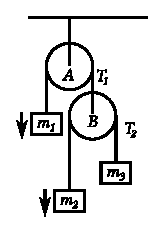
\includegraphics[width=3cm]{problem.eps}
		\vspace{-1cm}
	\end{wrapfigure}
	Let us consider the special case of $m_2 = m_3$. We can see that the accelerations then reduces to:
	\begin{align}
		a_1 &= \frac{(m_1-2m_2)g}{m_1+2m_2} \\
		a_2 = a_3 &= \frac{(2m_2-m_1)g}{m_1+2m_2} = -a_1
	\end{align}
	Indeed, this is what we would expect if we had attacked the problem by treating pulley $B$ and masses $m_2$ and $m_3$ as one combined mass in a normal pulley system around $A$. 
	
	As $m_2 = m_3$, there is also naturally no relative motion between $m_2$ and $m_3$.
	
	Notice how this is the solution if and only if $m_2 = m_3$. This is because this is the only case in which the center of mass of the system on the right accelerates at the same rate as pulley $B$ itself. 
	
	On top that, if $m_1 = m_2 + m_3$, the accelerations then reduces in this even more special case to:
	\begin{equation}
		a_1 = a_2 = a_3 = 0
	\end{equation}
	This makes absolute sense. If there is no difference in the masses on the left and right of the pulley, then there would be no net force on any of the masses and the whole system would be in equilibrium.
	
	\section*{Conclusion}
	There are usually 2 steps in solving all pulley problems that may be foreign to you (See Morin's):
	\begin{enumerate}
		\item Apply Newton's 2\textsuperscript{nd} Law
		\item Apply Conservation of String
	\end{enumerate}
	Applying these in the right way will yield the results we want. 
	
	\section*{Other ways}
	You may find online that there are other ways of doing this particular problem, including using the Lagrangian method. But that is beyond the scope of this. Feel free to explore these on your own time.
	
	\pagebreak
	
	\begin{appendices}
		\section{Conservation of String}
		\label{appdx:COS}
		\begin{wrapfigure}{r}{3cm}
			\centering
			\vspace{-0.7cm}
			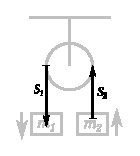
\includegraphics[width=2.5cm]{pulleyCOS.eps}
			\caption{A normal pulley}
			\label{fig:PconservationOfString}
		\end{wrapfigure}
		
		The entire principle behind the conservation of string is that the total length of string cannot change.
		
		For a simple pulley (Figure \ref{fig:PconservationOfString}), we notice that:
		\begin{equation*}
		S_1 + S_2 = L
		\end{equation*}
		where $S_1$ and $S_2$ are the displacements of $m_1$ and $m_2$ respectively, and $L$ is a constant equal to the length of the string used.
		
		Differentiating both sides of the equation with respect to time, 2 times\footnote{We are basically finding the rate of change of some variable, in this case the displacement $S$. The rate of change of a constant is naturally zero.}:
		\begingroup
		\addtolength{\jot}{0.7em}
		\begin{align*}
		\dod{}{t}\left(S_1 + S_2 \right) &= \dod{}{t}L \\
		\dod{S_1}{t} + \dod{S_2}{t} &= 0 \\
		\dod{}{t}\left(\dod{S_1}{t} + \dod{S_2}{t}\right) &= \dod{}{t} 0 \\
		\dod[2]{S_1}{t} + \dod[2]{S_2}{t} &= 0 \\[-0.5em]
		&\implies a_1 + a_2 = 0 \hspace{1em}\implies a_1 = -a_2 
		\end{align*}
		\endgroup
		
		And indeed we obtain the equation that we expect, that the acceleration $a_1$ is equal in magnitude, but opposite in direction to $a_2$. 
		
		\vfill
		
		\pagebreak
		
		\section{Solving the equations using Gaussian Elimination}
		\label{appdx:GES}
		We have the following system of linear equations:
		\begin{align*}
			m_1 a_1 + T_1 &= m_1 g \tag{\ref{eqn:m1a1}} \\
			m_2 a_2 + T_2 &= m_2 g \tag{\ref{eqn:m2a2}} \\
			m_3 a_3 + T_2 &= m_3 g \tag{\ref{eqn:m3a3}} \\
			T_1 - 2 T_2 &= 0 \tag{\ref{eqn:tension}} \\
			2a_1 + a_2 + a_3 &= 0 \tag{\ref{eqn:COS}}
		\end{align*}
		To solve the equation using \textit{Gaussian Elimination}, we first set up the following \textit{augmented matrix} using the coefficients of the variables in the equations:
		\begin{equation*}
			\begin{blockarray}{ccccccc}
			& a_1 & a_2 & a_3 & T_1 & T_2 \\
			\begin{block}{c[ccccc|c]}
			R_1 & m_1 & 0 & 0 & 1 & 0 & m_1g \\  
			R_2 & 0 & m_2 & 0 & 0 & 1 & m_2g \\
			R_3 & 0 & 0 & m_3 & 0 & 1 & m_3g \\
			R_4 & 0 & 0 & 0 & 1 & -2 & 0 \\
			R_5 & 2 & 1 & 1 & 0 & 0 & 0 \\
			\end{block}
			\end{blockarray}
		\end{equation*}
		We can then perform row operations in order to find its \textit{Reduced Row Echelon Form (RREF)} :
		\begin{align*}
			\begin{amatrix}{5}
			m_1 & 0 & 0 & 1 & 0 & m_1g \\  
			0 & m_2 & 0 & 0 & 1 & m_2g \\
			0 & 0 & m_3 & 0 & 1 & m_3g \\
			0 & 0 & 0 & 1 & -2 & 0 \\
			2 & 1 & 1 & 0 & 0 & 0			
			\end{amatrix}
			&\xrightarrow[]{\frac{R_1}{m_1}, \frac{R_2}{m_2}, \frac{R_3}{m_3}}
			\begin{amatrix}{5}
			1 & 0 & 0 & \frac{1}{m_1} & 0 & g \\  
			0 & 1 & 0 & 0 & \frac{1}{m_2} & g \\
			0 & 0 & 1 & 0 & \frac{1}{m_3} & g \\
			0 & 0 & 0 & 1 & -2 & 0 \\
			2 & 1 & 1 & 0 & 0 & 0			
			\end{amatrix} \\
			\xrightarrow[]{R_5 - 2R_1 - R_2 - R_3}
			&\begin{amatrix}{5}
			1 & 0 & 0 & \frac{1}{m_1} & 0 & g \\  
			0 & 1 & 0 & 0 & \frac{1}{m_2} & g \\
			0 & 0 & 1 & 0 & \frac{1}{m_3} & g \\
			0 & 0 & 0 & 1 & -2 & 0 \\
			0 & 0 & 0 & -\frac{2}{m_1} & -(\frac{1}{m_2} + \frac{1}{m_3}) & -4g			
			\end{amatrix} \\
			\xrightarrow[]{R_5 + \frac{2}{m_1} R_4}
			&\begin{amatrix}{5}
			1 & 0 & 0 & \frac{1}{m_1} & 0 & g \\  
			0 & 1 & 0 & 0 & \frac{1}{m_2} & g \\
			0 & 0 & 1 & 0 & \frac{1}{m_3} & g \\
			0 & 0 & 0 & 1 & -2 & 0 \\
			0 & 0 & 0 & 0 & -(\frac{1}{m_2} + \frac{1}{m_3} + \frac{4}{m_1}) & -4g			
			\end{amatrix} \\
			\xrightarrow[]{R_5 \div \left[-\left(\frac{1}{m_2} + \frac{1}{m_3} + \frac{4}{m_1}\right)\right]}
			&\begin{amatrix}{5}
			1 & 0 & 0 & \frac{1}{m_1} & 0 & g \\  
			0 & 1 & 0 & 0 & \frac{1}{m_2} & g \\
			0 & 0 & 1 & 0 & \frac{1}{m_3} & g \\
			0 & 0 & 0 & 1 & -2 & 0 \\
			0 & 0 & 0 & 0 & 1 & 4g/\left(\frac{1}{m_2} + \frac{1}{m_3} + \frac{4}{m_1}\right)
			\end{amatrix}
		\end{align*}
		\vspace{-2cm}
		\begin{align*}
			\xrightarrow[]{R_4 + 2R_5}
			&\begin{amatrix}{5}
			1 & 0 & 0 & \frac{1}{m_1} & 0 & g \\  
			0 & 1 & 0 & 0 & \frac{1}{m_2} & g \\
			0 & 0 & 1 & 0 & \frac{1}{m_3} & g \\
			0 & 0 & 0 & 1 & 0 & \frac{8g}{\frac{1}{m_2} + \frac{1}{m_3} + \frac{4}{m_1}} \\
			0 & 0 & 0 & 0 & 1 & \frac{4g}{\frac{1}{m_2} + \frac{1}{m_3} + \frac{4}{m_1}}
			\end{amatrix} \\
			\xrightarrow[R_2-\frac{1}{m_2}R_5,~R_3-\frac{1}{m_3}R_5]{R_1 - \frac{1}{m_1}R_4}
			&\begin{amatrix}{5}
			1 & 0 & 0 & 0 & 0 & g - \frac{8g}{m_1\left(\frac{1}{m_2} + \frac{1}{m_3} + \frac{4}{m_1}\right)} \\  
			0 & 1 & 0 & 0 & 0 & g - \frac{4g}{m_2\left(\frac{1}{m_2} + \frac{1}{m_3} + \frac{4}{m_1}\right)}\\
			0 & 0 & 1 & 0 & 0 & g - \frac{4g}{m_3\left(\frac{1}{m_2} + \frac{1}{m_3} + \frac{4}{m_1}\right)}\\[1em]
			0 & 0 & 0 & 1 & 0 & \frac{8g}{\frac{1}{m_2} + \frac{1}{m_3} + \frac{4}{m_1}} \\[1em]
			0 & 0 & 0 & 0 & 1 & \frac{4g}{\frac{1}{m_2} + \frac{1}{m_3} + \frac{4}{m_1}}
			\end{amatrix}
		\end{align*}
		For those that might be confused, these row operations\footnote{You can imagine row operations as taking one equation and subtracting/adding it to another equation, or multiplying it by a certain constant multiple. Doing it in the matrix form makes it easier and more versatile. } are not arbitrary. There are 3 steps in trying to obtain the RREF through Gaussian Elimination:
		\begin{enumerate}
			\item Form a triangle of zeros in the bottom left corner
			\textit{\item Reduce all coefficients to 1. }\footnote{This step can be moved around, so long as it is ultimately performed so that we obtain a diagonal matrix on the left.}
			\item Form a triangle of zeros in the top right corner
		\end{enumerate}
	
		After obtaining the RREF, we can convert these back to their equivalent system of linear equation to obtain the solution:
		\begin{align*}
			a_1 &= g - \frac{8g}{m_1\left(\frac{1}{m_2} + \frac{1}{m_3} \right) + 4} \\
			a_2 &= g - \frac{4g}{m_2\left( \frac{4}{m_1} + \frac{1}{m_3}\right) + 1} \\ 
			a_3 &= g - \frac{4g}{m_3\left(\frac{4}{m_3} + \frac{1}{m_2}\right) + 1} \\
			T_1 &= \frac{8g}{\frac{1}{m_2} + \frac{1}{m_3} + \frac{4}{m_1}} \\
			T_2 &= \frac{4g}{\frac{1}{m_2} + \frac{1}{m_3} + \frac{4}{m_1}}
		\end{align*}
		
		If you perform some tedious algebraic manipulations, we would obtain the same solutions as the one we previously found.
		\vfill
	\end{appendices}
\end{document}